% !Mode:: "TeX:UTF-8"
\chapter{云辅助的车辆网络功率控制与任务卸载} \label{chap:table}  %\cite{yaojianquan2009}

\section{引言}\label{section3-1} \label{chap:introduction}
云辅助移动边缘计算(C-MEC)为车载网络提供了丰富的计算资源,是一种前景广阔的任务卸载解决方案。本章提出了一种鲁棒的功率
控制和任务卸载方案,以卸载计算任务并最大化 C-MEC 网络的效用。然而,不确定的信道状态会严重影响卸载任务的传输稳定性。为
了模拟信道的不确定性,采用了一阶马尔可夫过程,并考虑了车辆的移动性。此外,由于频谱资源有限,假设信道重用会导致复杂的同
信道干扰。为了克服这些限制,对信号链路实施了概率约束,以确保通信质量。采用伯恩斯坦近似法将原始约束转化为可解约束。此外,
还进一步采用了块坐标下降(BCD)方法和连续凸近似(SCA)技术来解决非凸鲁棒性优化问题。为确定最优解,提出了一种鲁棒功率控
制和任务卸载调度算法。对提出的算法进行了数值仿真,以评估系统的性能。结果表明,与基准模型相比,该算法非常有效,尤其是在
信道不确定的通信环境中。移动边缘计算(MEC)和移动云计算(MCC)作为新兴的5G 网络的两种新架构,通常用于支持物联网设备的任
务卸载、特别是提供低延迟、高可靠性的计算服务。MEC 可以充当网络中心边缘的云服务提供商,提供存储、图像、缓存和第三方访问
功能,这不仅减轻了无线网络的带宽压力,还提供了低延迟、高可靠性的计算服务 \cite{基于车辆边缘计算的任务卸载策略研究}。
并且MEC 在网络中心的边缘,可以减少传输延迟,并为车辆分配计算资源,以缓解计算压力 \cite{CCO}。 然而,当计算任务要求较高时,
MEC 的计算资源仍显不足。由于高性能计算由云服务器提供,基于云的计算网络已被部署以满足爆炸式增长的计算卸载需求 \supercite{Towards2024,SurveyMEC2017,SurveyMEC2018,DistributedTask2024}。
然而,云计算中心往往远离主干道,导致云计算延迟较长并造成网络拥堵与隐私泄露等问题 \supercite{Qian2023, 曹宇慧车载边缘计算环境下任务协同卸载方法研究,云计算隐私10418975}。
在高动态车联网中,车辆传输的数据必须实时处理。因此,在网络架构中部署C-MEC,以提供丰富的计算资源并减少传输延迟。

本章提出了一种鲁棒的云功率控制和任务卸载算法,以辅助高动态车辆网络中的 MEC。 与现有的功率控制或资源分配计算方面的单边研
究不同,本章研究了一个非常强调协作的网络系统,并通过满足概率约束保证了通信延迟和计算延迟;在该框架中,车辆的服务质量(QoS)
也得到了保证。 综上所述,本章的主要贡献可概述如下:
%\begin{itemize}
%\item

(1) 考虑了用于计算卸载架构的实用 C-MEC 车辆网络。 由于 MEC 层部署在网络附近并具有计算能力,因此 MEC 层可作为车辆与云服务器之间的桥梁。 云计算层处理 MEC 层无法处理的对延迟不敏感的大规模数据。 这种网络结构缩短了传输时间,并提供了大量的计算资源。

(2) 采用一阶马尔可夫过程来处理 C-MEC 车辆网络环境高速移动引起的信道不确定性。 为了模拟C-MEC 车载网络的动态特性,采用Bernstein 方法逼近大规模动态车载网络环境中的非凸中断约束。

(3) 提出了一种处理传输任务的高效结构,并开发了一种鲁棒的功率控制和任务卸载调度算法,以接近最优解。 在 C-MEC 车辆网络下,当任务发起车辆无法独立完成任务时,利用 V2R 传输来减少延迟。 模拟验证了系统卸载效用的提高。
%\end{itemize}
\section{系统模型与问题描述}\label{section3-2}
本文研究的C-MEC 车载网络如图 \ref{F1} 所示,由MEC 层和云计算层分层计算卸载架构组成。众多车辆在RSU 的覆盖范围内被划分为多个地理区域,每个RSU 下覆盖一个小区,每个RSU 配备一台MEC 服务器,为车辆提供计算卸载服务。我们将移动系统中的两组车辆和MEC 服务器分别记为$\mathcal{V}=\left\{1,2,..., V\right\}$ 和$\mathcal{M}=\left\{1,2,..., M\right\}$。 高速移动无线通信链路称为 V2RSU (V2R)链路,固定有线连接链路称为 RSU 到云(R2C)链路。详细的卸载过程描述如下。首先,车辆通过无线接口向云发送卸载请求信息,其中包括所需的通信资源、任务 ID 和提交时间,以及任务的最大可容忍服务时间。其次,MEC 服务器根据接收到的请求信息进行调度,包括任务上传服务器和任务计算服务器。最后,任务上传后,任务被推送到服务器队列中,直到服务器执行任务。
% 此外,本文中使用的一些术语如表所示。
\begin{figure}[H]
\centering
\includegraphics[width=12cm]{figures//chap3//model2.eps}
\caption{C-MEC 系统模型图}
\label{F1}
\end{figure}

\subsection{通信模型}\label{section3-2-1}
由于车辆移动速度快,通信模式与传统的蜂窝通信不同。因此,很难直接获得 CSI。 其中,RSU 仅能准确获取车辆到 RSU 链路的大尺度衰落 $L^2$,而小尺度衰落 $h$ 受多普勒效应引起的快速信道变化影响较大。我们假设CSI 是通过信道估计获得的,因此,我们利用一阶高斯- 马尔可夫过程\cite{Kim2011} 对每个传输时间间隔内的小尺度衰落信道估计$h$ 建模如下,
\begin{eqnarray}\label{E1}
h=\xi{\widetilde{h}}+\sqrt{1-\xi^2}\zeta
\end{eqnarray}
我们假设估计的信道增益 $\widetilde{h}$ 表示对 $h$ 的估计,${\widetilde{h}}^2$ 是指数分布,具有单位平均值\cite{Sakr2014}。 此外,$\xi\in\left(0,1\right)$ 表示 V2R 链路上的相关系数,$\zeta$ 表示信道增益,其复高斯分布为 $\zeta\sim CN\left(0,\delta^2\right)$ ,与 $\widetilde{h}$ 无关。系数$\left(0<\zeta<1\right)$ 量化了两个连续时隙之间的信道相关性,我们假设所有车辆都存在相同的时间相关系数$\zeta$。Jakes 的衰落信道统计模型\cite{Kim2011} 指出:$\zeta=J_0\left(2\pi f_{max}T_s\right)$ ,其中$J_0$ 是第一类零阶贝塞尔函数。$f_{max}=\bar{\nu}f_c/c $ 是最大多普勒频率,其中 $\bar{\nu}$ 表示车辆速度,$f_c$ 表示 5.9 Ghz 的载波频率,$c=3\times{10}^8$m/s,$T_s$ 是周期反馈延迟。发射车和 RSU 都知道实际的 $\zeta$。

根据上述讨论,从第$ i$ 个车辆发射器到第 $j $ 个接收器的第$ k $ 个时隙内,有效链路和干扰链路的移动 V2R 信道功率增益用共享表达式表示:
\begin{eqnarray}\label{E2}
G_{i,j}^k={\widetilde{g}}_{i,j}^k+{\hat{g}}_{i,j}^k
\end{eqnarray}
其中 ${\widetilde{g}}_{i,j}^k=L_{i,j}^2{\widetilde{h}}_{i,j}^2\xi_{i,j}^2$ , ${\hat{g}}_{i,j}^k=L_{i,j}^2\left(1-\xi_{i,j}^2\right)\zeta_{i,j}^2\ $ ,$ {L_{i、 j}^k}^2 $
表示第 $k $ 个时隙的大规模衰减效应,包括阴影衰减和从道路上第 $i$ 个车辆发射器到第 $ j $ 个接收器的路径损耗。此外,${\hat{g}}_{i,j}^k$ 是观测值,${\widetilde{g}}_{i,j}^k$ 表示指数随机变量,参数为 $\frac{1}{L_{i,j}^k}^2({1-{\zeta_{i,j}^k}^2}) $ ,该参数基于 \cite{Xie2020}。

为了提高频谱利用率并实现多车联合通信,V2R 通信重复使用同一上行链路信道。换句话说,车辆 $j$ 和车辆 $i$ 共享同一个上行链路信道,从而导致它们之间产生干扰。在这种情况下,V2R 链路的信号干扰加噪声比(SINR)计算公式为,
\begin{eqnarray}\label{E3}
%\gamma_i\left(\mathbf{p}\right)=\frac{p_ig_{i,j}}{{\sum_{j=1,j\neq i}^{M}{p_jg_{j,i}}+\sigma^2}},
\gamma_i\left(\mathbf{p}\right)=\frac{p_ig_{i,m}}{{\sum_{j=1}^{M}{p_jg_{j,m}}+\sigma^2}}, m=1,2,\cdots ,M , i\in {{\mathcal{V}}_{m}}
\end{eqnarray}
% 其中,$p_j$ 表示第 j 个发射器车辆的发射功率,$\sigma^2$ 为背景噪声。因此,根据香农定理计算出车辆的确定性等效传输速率为,
其中,$g_{i,m}$ 表示 $i_{th}$ 车辆对其集群 RSU 的功率增益,而 ${p_jg_{j,m}}$ 表示其他集群车辆对当前 RSU 的干扰。
\begin{eqnarray}\label{E4}
%{R_i\left(\mathbf{p}\right)=\log}_2{\left(1+\frac{p_ig_{i,j}}{\sum_{j=1,j\neq i}^{M}{p_jg_{j,i}}+\sigma^2}\right)}.
{R_i\left(\mathbf{p}\right)=\log}_2{\left(1+ \gamma_i\left(\mathbf{p}\right) \right)}
\end{eqnarray}
当输入参数为 $d_{i,up}$ 时,车辆 $i$ 向上行链路发送任务输入时的传输时间定义为 $t_{i,up}$。

因此,每个 V2R 链路的上传时间可表述为,
\begin{eqnarray}\label{E6}
t_{i,up}=\frac{d_{i,up}}{WR_i\left(\mathbf{p}\right)}
\end{eqnarray}
其中,$W$ 表示多个 V2R 链路重复使用的信道带宽,$d_{i,up}$ 表示输入数据的大小,包括系统设置、程序代码和输入参数,这些数据是程序执行时必须传输的。

% 通信传输延迟是影响车载网络性能的一个重要因素 \cite{RAI}。 到 RSU 的数据包在传输前必须进入队列,其中传输速度为 $R_i$。 第i 个V2R 接收器的数据包到达过程遵循参数为$k_i$ 的泊松过程,数据包长度为参数为$\tau_i$ 的指数分布。由于基于$M/M/1$ 队列的方法可以保证车辆通信的可靠性,我们利用$M/M/1$ 模型对系统进行分析,并将预期时延表示为第i 条V2R 链路传输速率的函数,其表达式如下,  \cite{liu2021}
通信服务延迟严重影响了车载网络的性能 \cite{RAI}。 为确保高效传输,数据包在传输到 RSU 之前必须排队。 传输速度(用 $R_i$ 表示)受两个参数的影响:数据包到达过程和数据包长度。  第i 个V2R 接收器的数据包到达过程遵循参数为$k_i$ 的泊松过程,数据包长度为参数为$\tau_i$ 的指数分布。 由于基于$M/M/1$ 的排队方法可以保证车辆通信的可靠性 \cite{Guo2019},因此我们利用$M/M/1$ 模型对系统进行分析,并将预期时延表示为第$i$ 条V2R 链路传输速率的函数,其表达式如下、
\begin{eqnarray}\label{E7}
D_i=\frac{1}{{\tau_iR}_i-k_i}.
\end{eqnarray}

\subsection{车辆计算模型}\label{section3-2-2}
我们将处理车辆 $i$ 的 1 位输入数据所需的 CPU 周期数表示为 $c_0$ \cite{Zhang2017},它不可分割,无法分解为更小的组件 \cite{Saleem2021}。
我们认为,在$ \mathcal{V}$ 中,每辆车每次都有不同的计算任务,记作 $T_i$,由两个参数组成的元组来定义,即 $\langle d_{i,up}, c_{i,e}\rangle$,其中 $c_{i,e}$ [cycles] 指定了工作量 \cite{Tran2019}。 因此,完成任务的计算成本 $c_{i,e}$ 可以通过 $c_{0}*d_{i,up}$ 得到。每个任务都被卸载到 MEC 服务器,然后传输到云服务器。通过将计算任务卸载到 MEC 服务器,车辆可以获得更多计算资源。然而,在上行链路方向传输任务输入可能会消耗额外的时间。

每个 RSU 上的 MEC 服务器按时段为车辆提供计算卸载服务。计算资源由固定速率 $\bar{f}$ (即每秒 CPU 周期数)量化。第 $i $ 辆车将每个任务的输入数据上传到最近的 RSU。RSU 首先处理小规模、对延迟敏感的数据,然后将剩余数据转发给远程云服务器。{云服务器同时为多个 RSU 提供计算服务。RSU 可用的计算资源取决于从云服务器分配的计算速率 $f_i$,}即每秒 CPU 周期数。因此,计算卸载造成的延迟可计算为,
\begin{eqnarray}\label{E8}
t_{i,exe}=\frac{c_{i,e}}{\bar{f}+f_i}
\end{eqnarray}
\subsection{问题的定义}\label{section3-2-3}
\begin{comment}
\begin{table}[htbp!]
 \centering\small
 \Tablecaption{燕山大学硕士学位论文参考文献规则}\label{tab:ysubof}
\begin{tabular}{llr}
 \toprule
    论文版本    & 参考文献标准    & 实施年份(年)  \\
 \midrule
    旧版        & BF7714-87       & 1987            \\
    新版        & GBT7714-2005    & 2005            \\
 \bottomrule
 \end{tabular}
\end{table}
\end{comment}
如果计算速度为 $f_i$,则车辆 $i$ 因卸载而产生的总延迟时间为,
\begin{eqnarray}\label{E9}
 t_i=\frac{c_{i,e}}{\bar{f}+f_i}+T_c
\end{eqnarray}
其中,云服务器和 RSU 之间的传输延迟定义为 $T_c$,通常设为一个常量 \cite{Xiao2020}。 因此,任务完成时间的相对效用函数的特征为,
\begin{eqnarray}\label{E10}
U_{i,exe}=\frac{t_{max}-t_{i,exe}}{t_{max}}
\end{eqnarray}
其中,$t_{max}$ 为{任务完成可容忍阈值的最长时间}。换句话说,当任务同时在 MEC 服务器和云上执行时,每辆车都能通过最小化任务执行时间获得更大的效用。否则,就会产生相应的损失。因此,车辆 $i$ 的卸载效用定义为 $\frac{U_{i,exe}}{t_{i,up}}$,即单位时间内的卸载效用函数。

本节将功率控制和任务卸载表述为一个优化问题,试图最小化网络中所有车辆由延迟和传输速率组成的总系统成本。给定上行链路功率分配向量 $\mathbf{p}$ 和计算速率向量 $\mathbf{f}$ 后,系统效用被定义为所有车辆卸载效用的加权和。
\begin{eqnarray}\label{E12}
U=\sum_{i=1}^{M}\frac{U_{i,exe}}{t_{i,up}}
\end{eqnarray}
其中,$U$ 是更大的执行时间效用,上传时间成本较小。我们将鲁棒优化问题,即功率控制和任务卸载问题,表述为系统效用最大化问题,
\begin{align}
& \max\limits_{\mathbf{p},\mathbf{f}}\sum_{i=1}^{M}\frac{U_{i,exe}}{t_{i,up}}                                   \label{E3-13}\\
\text { s.t. }
& \textrm{Pr}\left\{\gamma_i\geq\gamma_{th}\right\}\geq1-\varepsilon_1                                         \tag{\ref{E3-13}{-1}}      \label{E3-13-1}\\  % 信噪比中断概率约束
& \textrm{Pr}\left\{\frac{1}{\tau_iR_i-k_i}+\frac{c_{i,e}}{\bar{f}+f_i}\le D_{max}\right\}\geq1-\varepsilon_2  \tag{\ref{E3-13}{-2}}      \label{E3-13-2}\\  % 功率阈值
& \sum_{i=1}^{N}f_i\le f_{total}                                                                                \tag{\ref{E3-13}{-3}}      \label{E3-13-3}\\  % 时隙分配加起来是一
& 0\le p_i\le p_{max}                                                                                          \tag{\ref{E3-13}{-4}}      \label{E3-13-4} % 这个是时隙的约束
%& q_U^{n\mathrm{\ }+1}-q_U^{n\mathrm{\ }}\le tV_{max}, \forall m         \tag{\ref{E2-13end}{-5}}      \label{E2-13end5}    % 无人机飞行轨迹
\end{align}
其中,$U$ 表示网络效用。\eqref{E3-13} 中的约束条件解释如下: 约束条件 \eqref{E3-13-1} 保证了车辆的 QoS 要求。然而,网络拓扑结构的时变会导致大量计算。在车辆通信场景中,实时 SINR 难以量化获取。由于 CSI 反馈的时间间隔非常小,因此用长期 SINR 代替实时 SINR。 我们用 $\gamma_i$ 表示第$i$ 个 V2R {链路的平均 SINR,使用较小的 CSI 反馈时间间隔}。为确保任务成功卸载到 RSU,SINR 必须大于 SINR 阈值 \cite{liu2021}。$\gamma_{th}$ 是检测 V2R 链路通信的 SINR 阈值。$\textrm{Pr}\left\{\cdot\right\}$ 定义了输入 SINR 的概率。中断概率约束保证了车辆链路的可靠性。$D_{max}$ 表示第 $i$ 个 V2R 链路在数据传输过程中允许的最大延迟。此外,$\varepsilon_1$ 和$\varepsilon_2$ 分别是与SINR 和延迟约束相关的中断概率阈值,其中$\varepsilon_1,\varepsilon_2\in\left(0,1\right)$。 约束 \eqref{E3-13-2} 表示通信和计算的总延迟大于延迟阈值。约束 \eqref{E3-13-3} 确保云服务器必须为与其相关联的 RSU 分配计算资源,约束 \eqref{E3-13-3} 还确保分配给所有相关联 RSU 的总计算资源不得超过云服务器的计算能力。因此,特定边缘云所服务的应用数量必须低于其容量。在约束条件 \eqref{E3-13-4} 中,$p_{max}$ 是车辆通信网络中发射车辆的最大发射功率,且发射功率大于零。

\begin{comment}
实现代码如下:
\end{comment}
\section{功率控制与任务资源分配问题的求解}\label{section3-3}
在本节中,我们提出了一种基于 BCD 的算法来求解优化问题 \eqref{E3-13}。BCD 方法将复杂的原问题分解为一系列较简单的子问题。BCD 方法首先将所有变量分成两块,交替优化。

为了解决 \eqref{E3-13} 问题,可以通过固定计算率向量 $\mathbf{f}$ 的优化变量来优化问题。该问题通过交替优化两个子问题来解决。去掉向量 $\mathbf{f}$ 后,问题 \eqref{E3-13-1} 可以转化为下面的问题,
\begin{align}
& \textbf{P1}:\max\limits_{\mathbf{p}}\sum_{i=1}^{M}\frac{U_{i,exe}}{t_{i,up}}                                  \label{E3-14}\\
\text { s.t. }
& \textrm{Pr}\left\{\gamma_i\geq\gamma_{th}\right\}\geq1-\varepsilon_1                                         \tag{\ref{E3-14}{-1}}      \label{E3-14-1}\\  % 信噪比中断概率约束
& \textrm{Pr}\left\{\frac{1}{\tau_iR_i-k_i}+\frac{c_{i,e}}{\bar{f}+f_i}\le D_{max}\right\}\geq1-\varepsilon_2  \tag{\ref{E3-14}{-2}}      \label{E3-14-2}\\  % 功率阈值
& 0\le p_i\le p_{max}                                                                                          \tag{\ref{E3-14}{-3}}      \label{E3-14-3}  %\\  % 时隙分配加起来是一
%& 0\le p_i\le p_{max},                                                                                          \tag{\ref{E3-13}{-4}}      \label{E3-13-4} % 这个是时隙的约束
%& q_U^{n\mathrm{\ }+1}-q_U^{n\mathrm{\ }}\le tV_{max}, \forall m         \tag{\ref{E2-13end}{-5}}      \label{E2-13end5}    % 无人机飞行轨迹
\end{align}

\subsection{目标方程中的连续凸逼近方法}\label{section3-3-1}
由于$t_{i,up}$ 中的香农定理的形式,目标函数\eqref{E3-14} 是对数形式,因此\eqref{E3-14-1} 是一个非凸和非确定多项式困难(NP-hard)问题。这里使用 SCA 方法将问题 \eqref{E3-14-1} 简化为可解问题。利用近似约束来近似原始函数如下,
\begin{eqnarray}\label{E15}
\begin{array}{ll}
\alpha \ln{\left(z\right)}+\beta\le \ln{\left(1+z\right)},\\
\end{array}
\end{eqnarray}
其中 $\alpha=\frac{z_0}{1+z_0}$ 并且 $\beta=\ln{\left(1+z_0\right)}-\frac{z_0}{1+z_0}\ln{\left(z_0\right)}$。 \eqref{E15} 中的每个项都可以通过连续凸近似转换为 $A_k\ln\left(\gamma_k\left(e^{\widetilde{\mathbf{p}}}\right)\right)+B_k$ 。 其中,$A_k$ 和$B_k$ 分别选为$A_k=\gamma_i/\left(1+\gamma_i\right)$ 和$B_k=\ln{\left(1+\gamma_i\right)}-A_k\ln{\left(\gamma_i\right)}$,其中$A_k=1$,$B_k=0$。目标函数的每项都可以写成如下,
\begin{eqnarray}\label{E16}
\frac{1}{\ln{2}}\sum_{i=1}^{M}{\frac{U_{i,exe}}{d_{i,up}}\left.\left[{A_k\ln{\left(\gamma\left(p\right)\right)}+B}_k\right.\right]},
\end{eqnarray}
由于 \eqref{E3-14} 中的目标函数是 SINR 的分数,因此不容易直接计算。因此,我们使用变量替换法,即 ${\hat{p}}_i=\ln{p_i}$,
$p_i=e^{{\hat{p}}_i}$, and ${\hat{p}}_i\le \ln{p_{max}},\ \forall\ \ 1\le i\le M$
\begin{eqnarray}\label{E17}
U=\max\frac{1}{\ln{2}}\sum_{i=1}^{M}\left.\frac{U_{i,exe}}{d_{i,up}}\left[{A_k\ln{\left(\gamma\left(e^{\widetilde{P}}\right)\right)}+B}_k\right.\right]
\end{eqnarray}

\begin{comment}
\begin{table}[htbp!]
\centering\small
\Tablecaption{带有合并列的三线表}\label{tab:test}  % 合并列通常见于表格的第一行,在适当的位置使用\verb|\multicolumn| 命令即可。
\begin{tabular}{llr} \toprule
\multicolumn{2}{c}{Item} \\ \cmidrule(r){1-2}
Animal & Description & Price (\$)\\ \midrule
Gnat & per gram & 13.65 \\
& each & 0.01 \\
Gnu & stuffed & 92.50 \\
Emu & stuffed & 33.33 \\
Armadillo & frozen & 8.99 \\ \bottomrule
\end{tabular}
\end{table}
\end{comment}


\subsection{中断概率的近似}\label{section3-3-2}
\begin{comment}
\begin{table}[htbp!]
\end{comment}
由于 \eqref{E3-14-1} 是不确定的,而目标函数 \eqref{E3-14} 又是一个非凸问题,因此优化 \eqref{E3-14} 十分困难。有必要设计一种复杂度较低的算法来求解 \eqref{E3-14}。 为了描述不确定信道增益,考虑到快速衰落,采用统计约束来描述不确定性 \eqref{E3-14-1}。 为了进一步简化 \eqref{E3-14-1},引入了矩阵形式。信道增益的一般形式描述为:
\begin{eqnarray}\label{E18}
\textrm{Pr}\left\{\left(\textbf{G}_m\right)^Te^{\widetilde{p}}+\sigma^2\le0\right\}\geq1-\varepsilon_1
\end{eqnarray}
其中 $\textbf{G}_m=\left[G_{1,m},G_{2,m},\ldots,-\frac{G_{m,m}}{\gamma_{th}},\ldots,G_{M,m}\right]^T$。
此外,还采用伯恩斯坦方法来近似考虑信道不确定性的概率约束。

%\begin{theorem}
所有 V2R 链路的中断概率表示为 $\textrm{Pr}\left\{\gamma_i\geq\gamma_{th}\right\}\geq1-\varepsilon_1$
可以重新表述为可分离的约束条件,
\begin{eqnarray}\label{E19}
\!\!\!\sigma^2+\!\sum_{i\neq j}^{M}{\chi_{i,j}e^{{\widetilde{p}}_i}}+\sqrt{2\ln\left(\frac{1}{\varepsilon_1}\right)}\left(\sum_{i\neq j}^{M}\left(\sigma_{i,j}\beta_{i,j}p_i\right)^2\right)^\frac{1}{2}\!\!\!\!\!\le0
\end{eqnarray}
其中 $\chi_{i,j}=\mu_{i,j}^+\alpha_{i,j}+\beta_{i,j}+g_{i,j}$. 参数(即 $\sigma_{i,j}$ 和 $\alpha_{i,j}$)在 \cite{CCO} 中被推导为正值。假设 $G_{i,j}$ 的截断分布具有有界范围 $\left[{\widetilde{g}}_{i,j}^k+\alpha_{i,j},{\widetilde{g}}_{i,j}^k+\beta_{i,j}\right]$,${\widetilde{g}}_{i,j}^k$ 是 $G_{i,j}$ 的估计值。常数 $\alpha_{i,j}=\frac{1}{2}\left(b_{i,j}-a_{i,j}\right)$, $\beta_{i,j}=\frac{1}{2}\left(b_{i,j}+a_{i,j}\right)$ 用于将范围归一化为 $\left[-1,1\right]$ 如下,
\begin{eqnarray}\label{E20}
\xi_{i,j}=\frac{G_{i,j}-{\widetilde{g}}_{i,j}^k-\beta_{i,j}}{\alpha_{i,j}}\in\left[-1,1\right]
\end{eqnarray}
%\end{theorem}

在 \eqref{E19} 的最后一项中,变量 $p_i$ 是非线性耦合的。因此,当 $k$ 增加且车辆数量较多时,用伯恩斯坦方法确定一个可接受的良好解 \eqref{E3-14-1} 非常耗时。因此,有必要为 $\mathbb{R}^k$ 中的任意 $\mathbf{x}$ 引入一个 $\ell_2$ 准则近似问题。因此,包含向量 $\mathbf{x}=\left[\sigma_{i,1}\beta_{i,1}p_i,\cdots,\sigma_{i,M}\beta_{i,M}p_i\right]$ 进一步近似为 $\parallel x\parallel_2 \le \parallel x\parallel_1$. \eqref{E3-14} 中的约束条件被进一步表述为 \eqref{E21},复杂度降低,可靠性提高。
\begin{eqnarray}\label{E21}
\sigma^2+\sum_{i\neq j}^{M}{\chi_{i,j}e^{{\widetilde{p}}_i}}+\sqrt{2\ln\left(\frac{1}{\varepsilon_1}\right)}\sum_{i\neq j}^{M}{\left|\sigma_{i,j}\beta_{i,j}\right|e^{{\widetilde{p}}_i}}\le0
\end{eqnarray}

为了得到问题 \eqref{E21} 的简单形式,我们定义,
\begin{eqnarray}\label{E22}
\ \mathrm{\Pi}_i=\sigma^2+\sqrt{2\ln\left(\frac{1}{\varepsilon_1}\right)}\sum_{i\neq j}^{M}{\left|\sigma_{i,j}\beta_{i,j}\right|e^{{\widetilde{p}}_i}}
\end{eqnarray}

利用积分变换法重新表述了约束条件 \eqref{E3-14-2}。 根据约束条件 \eqref{E3-14-2},$X={\widetilde{h}}^2$ 是一个具有单位均值的指数随机变量,即 其中 $D_{max}=D_1+D_2 $,$D_1=\frac{1}{\tau_iR_i-k_i} $,$D_2=\frac{c_{i,e}}{f_i} $。 我们可以确定通信延迟概率的可行功率区域如下,
\begin{eqnarray}\label{E23}
\left.\left[\ln\left(1-\varepsilon_2\right)-{\hat{g}}_{i,j}^k\right.\right]e^{{\widetilde{p}}_i}+D^\ast\ \le0
\end{eqnarray}
证明求解过程如下,
\begin{equation}\label{E24}
\begin{array}{ll}
\textrm{Pr}\left\{\frac{1}{\tau_iR_i-k_i}+\frac{c_{i,e}}{f_i}\le D_{max}\right\}\\
=\textrm{Pr}\left\{R_i\geq\frac{1}{R_i\left(D_{max}-D_2\right)}+\frac{k_i}{\tau_i}\right\}\\
\!\le1\!-\!\textrm{Pr}\left\{p_i{\widetilde{g}}_{i,j}^k\le\left(I_{th}+\sigma^2\right)2^\frac{1+k_i\left(D_{max}-D_2\right)}{\tau_i\left(D_{max}-D_2\right)}-p_i{\hat{g}}_{i,j}^k\right\}\\
=\!1\!-\!\int_{0}^{\left(I_{th}+\sigma^2\right)2^\frac{1+k_i\left(D_{max}-D_2\right)}{\tau_i\left(D_{max}-D_2\right)}-p_i{\hat{g}}_{i,j}^k}{e^{-x}dx}\!\geq\!1-\varepsilon_2
\end{array}
\end{equation}
不等式函数 \eqref{E24} 等价于 \eqref{E25} 为,
\begin{eqnarray}\label{E25}
\left.\left[\ln\left(1-\varepsilon_2\right)-{\hat{g}}_{i,j}^k\right.\right]e^{{\widetilde{p}}_i}+D^\ast\ \le0
\end{eqnarray}
其中 $D^\ast=\left(I_{th}+\sigma^2\right)2^\frac{1+k_i\left(D_{max}-D_2\right)}{\tau_i\left(D_{max}-D_2\right)}$。

因此,将方程 \eqref{E3-26} 给出的鲁棒功率控制的确定性优化问题进行变换,我们可以将目标函数、停电概率约束和延迟约束重新表述如下:
\begin{align}
&\textbf{P1}:\max\limits_{\mathbf{p}}\frac{1}{\ln{2}}\sum_{i=1}^{M}\left.\frac{U_{i,exe}}{d_{i,up}}
\left[{A_k\ln{\left(\gamma\left(e^{\widetilde{P}}\right)\right)}+B}_k\!\!\right.\right]                         \label{E3-26}\\
\text { s.t. }
& \sum_{i=1}^{M}{\chi_{i,j}e^{{\widetilde{p}}_i}}+\mathrm{\Pi}_i\le0                                           \tag{\ref{E3-26}{-1}}      \label{E3-26-1}\\  % 信噪比中断概率约束
& \left.\left[\ln\left(1-\varepsilon_2\right)-{\hat{g}}_{i,j}^k\right.\right]e^{{\widetilde{p}}_i}+D^\ast\le0  \tag{\ref{E3-26}{-2}}      \label{E3-26-2}\\  % 功率阈值
& -\infty\le{\widetilde{p}}_i\le \ln{p_{i,max}}                                                                \tag{\ref{E3-26}{-3}}      \label{E3-26-3}  %\\  % 时隙分配加起来是一
\end{align}
\subsection{优化功率问题}\label{section3-3-3}
为了解决问题 \eqref{E3-26},我们使用了一种迭代算法,即拉格朗日法,当给出两个系数 $X_i$ 和 $Y_i$ 时,最大化原目标的下限。对这两个系数进行更新,以保证下限性能的单调增长。

因此,具有固定系数 $X_i$ 和 $Y_i$ 的 \eqref{E3-26} 的拉格朗日函数可表述为:
\begin{comment}
\begin{align}\label{E27}  % 没有左对齐的公式
L\left(\widetilde{\mathbf{p}},\lambda,\mu\right)=\frac{1}{\ln{2}}\sum_{i=1}^{M}{\frac{U_{i,exe}}{d_{i,up}}\left[A_k\ln{\left({\bar{\gamma}}_k\left(e^{\widetilde{\mathbf{p}}}\right)\right)}+B_k\right]}\\
\notag-\mu_k\Big[\left(\ln\left(1-\varepsilon_2\right)-{\hat{g}}_{i,j}^k\right)e^{{\widetilde{p}}_i}+D^\ast\Big]\\
-\lambda_k\Big[\sum_{i=1}^{M}{\chi_{i,j}e^{{\widetilde{p}}_i}}{+\mathrm{\Pi}}_i\Big]\notag,
\end{align}
\end{comment}

\begin{align}\label{E27}
L\left(\widetilde{\mathbf{p}},\lambda,\mu\right)&=\frac{1}{\ln{2}}\sum_{i=1}^{M}{\frac{U_{i,exe}}{d_{i,up}}\left[A_k\ln{\left({\bar{\gamma}}_k\left(e^{\widetilde{\mathbf{p}}}\right)\right)}+B_k\right]}\\
&\notag-\mu_k\Big[\left(\ln\left(1-\varepsilon_2\right)-{\hat{g}}_{i,j}^k\right)e^{{\widetilde{p}}_i}+D^\ast\Big]\\
&-\lambda_k\Big[\sum_{i=1}^{M}{\chi_{i,j}e^{{\widetilde{p}}_i}}{+\mathrm{\Pi}}_i\Big]\notag
\end{align}
其中 $\lambda_k$ 和 $\mu_k$ 是拉格朗日乘数,分别为 $\lambda_k\geq0$ 和 $\mu_k\geq0$ 。

微分方程 \eqref{E28} 用于求解迭代函数的幂向量 $\mathbf{p}$ 。
\begin{comment}
\begin{align}\label{E28}
\frac{\partial L\left(\mathbf{p},\lambda,\mu\right)}{\partial p_i}=A_i-\Bigl[\sum_{j=1,j\neq i}^{M}\left(A_j\frac{{\bar{\gamma}}_j\left(e^{\widetilde{p}}\right){\bar{G}}_{k,j}}{e^{{\widetilde{p}}_j}{\bar{G}}_{j,j}}\right)\\
+\lambda_i\mathrm{\Pi}_ie^{-{\widetilde{p}}_i}+\mu_i{\hat{g}}_{i,j}^k\Bigl]e^{{\widetilde{p}}_i}=0\notag,
\end{align}
\end{comment}
\begin{align}\label{E28}
\frac{\partial L\left(\mathbf{p},\lambda,\mu\right)}{\partial p_i}=A_i-\Bigl[\sum_{j=1,j\neq i}^{M}\left(A_j\frac{{\bar{\gamma}}_j\left(e^{\widetilde{p}}\right){\bar{G}}_{k,j}}{e^{{\widetilde{p}}_j}{\bar{G}}_{j,j}}\right)
+\lambda_i\mathrm{\Pi}_ie^{-{\widetilde{p}}_i}+\mu_i{\hat{g}}_{i,j}^k\Bigl]e^{{\widetilde{p}}_i}=0
\end{align}
根据 \eqref{E28},功率分配通过以下方式迭代更新,
\begin{comment}
\begin{align}\label{E29}
{\widetilde{p}}^{\left(t+1\right)}=\Big[\ln{A_i}+\ln\left(\sum_{j=1,j\neq i}^{M}\left(A_j\frac{{\bar{\gamma}}_j\left(e^{\widetilde{p}}\right){\bar{G}}_{k,j}}{e^{{\widetilde{p}}_j}{\bar{G}}_{j,j}}\right)
\notag\Big.\notag\right.\\
\phantom{=\;\;}\Big.+\lambda_i\mathrm{\Pi}_ie^{-{\widetilde{p}}_i}\Big.+\mu_i\hat{g}\Big)
\Big]_{-\infty}^{\ln{p_{max}}},
\end{align}
\end{comment}
\begin{align}\label{E29}
{\widetilde{p}}^{\left(t+1\right)}=\Big[\ln{A_i}+\ln\left(\sum_{j=1,j\neq i}^{M}\left(A_j\frac{{\bar{\gamma}}_j\left(e^{\widetilde{p}}\right){\bar{G}}_{k,j}}{e^{{\widetilde{p}}_j}{\bar{G}}_{j,j}}\right)\Big.\right.\phantom{=\;\;}\Big.\!\!\!\!\!\!\!\!\!\!\!+\lambda_i\mathrm{\Pi}_ie^{-{\widetilde{p}}_i}\Big.+\mu_i\hat{g}\Big)
\Big]_{-\infty}^{\ln{p_{max}}}
\end{align}

我们可以用次梯度法更新拉格朗日乘数 $\lambda$ 和 $\mu$ ,具体方法如下:
\begin{equation}\label{E30}
\lambda_i^{\left(t+1\right)}=\left[\lambda_i^{\left(t\right)}+K_\lambda^{\left(t\right)}\left(\sum_{j\neq i}^{M}{\chi_{i,j}e^{{\widetilde{p}}_j}}+\mathrm{\Pi}_i\right)\right]^+
\end{equation}
\begin{equation}\label{E31}
\mu_{i,j}^{\left(t+1\right)}=\!\left[\mu_{i,j}^{\left(t\right)}+\!K_\mu\!\left(\left(\ln\left(1-\varepsilon_2\right)-{\hat{g}}_{i,j}^k\right)e^{{\widetilde{p}}_i}+D^\ast\right)\right]^+
\end{equation}
其中 $K_\lambda$ 和 $K_\mu$ 代表拉格朗日乘法器的步长,$K_\lambda\geq0$ 和 $K_\mu\geq0$。 变量 $t$ 是迭代指数,变量 $x$ 的正部分定义为 $\left[x\right]^+=\max{\left[0,x\right]} $ 。
\subsection{计算资源分配}\label{section3-3-4}
在得到最优向量 $\mathbf{p}$ 之后,与向量 $\mathbf{f}$ 有关的问题被重新表述为,
\begin{align}
& \textbf{P2}:\max\limits_{\mathbf{f}}\sum_{i=1}^{N}\frac{U_{i,exe}}{t_{i,up}}                                      \label{E3-32}\\
\text { s.t. }
& \textrm{Pr}\left\{\frac{1}{\tau_iR_i-k_i}+\frac{c_{i,e}}{\bar{f}+f_i}\le \!\!D_{max}\right\}\geq1-\varepsilon_2  \tag{\ref{E3-32}{-1}}      \label{E3-32-1}\\  % 信噪比中断概率约束
& \sum_{i=1}^{N}f_i\le f_{total}                                                                                   \tag{\ref{E3-32}{-2}}      \label{E3-32-2}  % 功率阈值
%& -\infty\le{\widetilde{p}}_i\le \ln{p_{i,max}}.                                                                \tag{\ref{E3-32}{-3}}      \label{E3-32-3}  %\\  % 时隙分配加起来是一
\end{align}
注意到 \eqref{E3-32-1} 和 \eqref{E3-32-2} 中的约束条件是凸的。通过使用 $f_i$ 的二阶导数,采用拉格朗日函数来确定最优计算资源。因此,\eqref{E3-32} 的拉格朗日函数表述如下:
\begin{comment}
\begin{equation}\label{E33}
\begin{aligned}
Q\left(\mathbf{f},\xi,\varphi\right)=\frac{1}{\ln{2}}\sum_{i=1}^{M}\frac{R_i\left(P\right)}{ d_{i,up}}
\left[1-
\left(\frac{c_{i,e}}{t_{max}\left(\bar{f}+f_i\right)}
\right.\right.\\
\left.\left.
+\frac{T_c}{t_{max}}
\right)
\right]-\xi_k\left(\frac{1}{\tau_iR_i-\lambda_i}+\frac{c_{i,e}}{\bar{f}+f_i}-D_{max}\right)\\
-\varphi_k\left[\sum_{i=1}^{M}f_i-f_{total}\right].
\end{aligned}
\end{equation}
\end{comment}
\begin{equation}\label{E33}
\begin{aligned}
Q\left(\mathbf{f},\xi,\varphi\right)=\frac{1}{\ln{2}}\sum_{i=1}^{M}\frac{R_i\left(P\right)}{ d_{i,up}}
\left[1-
\left(\frac{c_{i,e}}{t_{max}\left(\bar{f}+f_i\right)}
\right.\right.
\left.\left.
+\frac{T_c}{t_{max}}
\right)
\right]\\
-\xi_k\left(\frac{1}{\tau_iR_i-\lambda_i}+\frac{c_{i,e}}{\bar{f}+f_i}-D_{max}\right)
-\varphi_k\left[\sum_{i=1}^{M}f_i-f_{total}\right]
\end{aligned}
\end{equation}
为了证明 \eqref{E3-32-1} 的凹性,我们考虑了$Q\left(\mathbf{f},\xi,\varphi\right)$ 关于$f_i$ 的一阶导数,
\begin{equation}\label{E34}
\!\!\frac{\partial Q\left(\mathbf{f},\xi,\varphi\right)}{\partial f_i}=\frac{c_{i,e}}{\ln{2} d_{i,up}t_{max}\left(\bar{f}+f_i\right)^2}=\frac{\mathrm{\Omega}_i}{\left(\bar{f}+f_i\right)^2}
\end{equation}
其中 $\mathrm{\Omega}_i=\frac{c_{i,e}}{\ln{2}d_{i,up}t_{max}}$, 二阶偏导数为,
\begin{equation}\label{E35}
\frac{\partial^2Q}{\partial f_i^2}=-\frac{2\cdot\mathrm{\Omega}_i}{\left(\bar{f}+f_i\right)^3}\le0
\end{equation}
其中 $Q\left(\mathbf{f},\xi,\varphi\right)$ 关于 $f_i$ 的二阶导数总是小于零。因此,$Q\left(\mathbf{f},\xi,\varphi\right)$ 是一个关于 $f_i$ 的凹函数。因此,\eqref{E3-32} 是一个凸优化问题,可以用卡鲁什$-$ 库恩$-$ 塔克条件求解。
\begin{equation}\label{E36}
\frac{\partial\left(\mathbf{f},\xi,\varphi\right)}{\partial f_i}=\frac{\mathrm{\Omega}_iR_i\left(P\right)}{\left(\bar{f}+f_i\right)^2}-\xi_k\frac{c_{i,e}}{\left(\bar{f}+f_i\right)^2}-\sum_{i=1}^{N}\varphi_k=0
\end{equation}
让$\frac{\partial \left(\mathbf{f},\xi,\varphi\right)}{\partial f_i}=0$,最佳计算资源分配为,
\begin{equation}\label{E37}
{f_i}^\ast=\sqrt{\frac{\mathrm{\Omega}_yR_i\left(P\right)-{c_{i,e}\xi}_k}{\sum_{i=1}^{N}\varphi_k}}-\bar{f}
\end{equation}
根据 \eqref{E37},第 $(t+1)$ 次迭代的最优计算率分配为,
\begin{equation}\label{E38}
{\tilde{f}}^{\left(t+1\right)}=\left[\sqrt{\frac{\mathrm{\Omega}_yR_i\left(P\right)
-{c_{i,e}\xi}_k}{\sum_{i=1}^{M}\varphi_k}}-\bar{f}\right]_0^{f_{total}\ }
\end{equation}
第$(t+1)$ 次迭代时的拉格朗日乘数 $\eta$, $\xi_i^{\left(t+1\right)}$ 和 $\varphi_{i,j}^{\left(t+1\right)}$ 是通过子梯度法更新的,具体方法如下,
\begin{equation}\label{E39}
\xi_i^{\left(t+1\right)}=\left[\xi_i^{\left(t\right)}\!+\!K_\xi^{\left(t\right)}\!\left(\frac{1}{\tau_iR_i
-\lambda_i}\!+\!\frac{c_{i,e}}{\bar{f}+f_i}\!-\!D_{max}\!\right)\!\right]^+
\end{equation}
\begin{equation}
\varphi_{i,j}^{\left(t+1\right)}=\left[\varphi_{i,j}^{\left(t\right)}+K_\varphi\left(\sum_{i=1}^{M}f_i
-f_{total}\right)\right]^+
\end{equation}
\section{算法与仿真验证}\label{section3-4}
\subsection{鲁棒的功率控制任务卸载调度算法}\label{section3-4-1}
在将原问题转化为两个凸子问题后,提出了另一种迭代算法来解决这两个凸子问题,该算法总结为算法3-1。
首先通过初始化的拉格朗日乘子$\lambda, \mu$ 以及物理初值求解第二个子问题的最优解,然后将求得最优解带入第一个子问题,如此反复迭代求解最终的最优值。

\begin{tabular*}{\hsize}{@{\extracolsep{\fill}}l l l l}
    \toprule
    算法3-1 鲁棒的功率控制任务卸载调度算法                                               \\
    \midrule
    Step1: 开始。                                                                      \\
    Step2: 初始化最大迭代次数$\mathcal{T}_{max}$ 和迭代初值 $\mathbf{f}$.              \\
    Step3: 初始化$\lambda, \mu$ 和 $\mathbf{f}$ 的可行解。                              \\ %, $n \in [1,2,...,N]$
    Step4: 求解问题 $\mathbf{P1}$,并得到最优解  ${{\tilde{p}}^{(t+1)}}$               \\%                                   ${\tilde{p}}^{\left(t+1\right)}$。 \\
    Step5: 初始化$\xi, \varphi$ 和 $\mathbf{p}$ 的可行解。                             \\
    Step6: 求解问题 $\mathbf{P2}$,并得到最优解 ${\widetilde{f}}^{\left(t+1\right)}$。 \\
    Step7: 重复执行Step5 至Step8,直到满足算法收敛或 $t\geq\mathcal{T}_{max}$。         \\
    Step8: 输出$\mathbf{f},\mathbf{p}$。                                               \\
    Step9: 结束。                                                                      \\
    \bottomrule
\end{tabular*}

算法3-1 的时间复杂度由其重复-until 循环中的最大循环次数$\mathcal{T}_{max}$ 决定。由于算法3-1 涉及 $V$ 集群进行功率迭代优化,其计算复杂度为 $O(V\mathcal{T}_{max})$。
\begin{comment}
\begin{table}[htbp!]
	\centering\small
	\Tablecaption{The relation of $E({{L}_{q}})$ with ${{p}_{2}}$ and $\theta$}\label{tab.2}
	\begin{tabular*}{\columnwidth}{@{\extracolsep{\fill}}@{~~}cccccccc@{~~}}
		\toprule
		\multicolumn{7}{c}{ \hspace{2cm} The expected waiting queue length $E({{L}_{q}})$}\\
		\cline{2-8}
		\raisebox{1ex}[0pt]{$\theta$}  &$p_2=0.1$     &$p_2=0.15$  &$p_2=0.2$   &$p_2=0.25$
        &$p_2=0.3$  &$p_2=0.35$   &$p_2=0.4$\\
		\midrule
		0.3     &16.4830  &5.1232   &2.9232   &1.9704   &1.4339   &1.0886   &0.8479\\
		0.5     &9.0488   &3.7848   &2.2906   &1.5839   &1.1723   &1.9035   &0.7146 \\
		0.7     &7.4321   &3.3256   &2.0528   &1.4338   &1.0686   &0.8291   &0.6607 \\
		\bottomrule
	\end{tabular*}	
\end{table}
\end{comment}
\subsection{仿真分析}\label{section3-4-2}
本节将通过数值仿真对算法3-1 的性能进行评估。我们将一个基于 MEC 的车载网络系统作为基本仿真场景,该系统在给定时隙内由五个集群组成。主要系统参数如表 \ref{biao3-1} 所示。在数值仿真中,
带宽 $W$ 设置为 10 MHz。 系统假设车辆和 RSU 都只使用一根天线进行发射和接收。此外,我们还假设车辆的速度在参考时间间隔内几乎没有变化。除非另有说明,路径损耗模型假定为 $d^{-\theta}$。

\begin{table}[htbp!]
 \centering\small
 \renewcommand\arraystretch{1.5}   %latex 三线表中各行间隔
 \Tablecaption{系统仿真参数}\label{biao3-1}
\begin{tabular*}{\hsize}{@{\extracolsep{\fill}}c c c c}
 \toprule
    \qquad\qquad 符号            &\qquad\qquad 参数                & \qquad\qquad 数值         \\
 \midrule
    \qquad\qquad $R_a$           &\qquad\qquad 基站的通信范围      & \qquad\qquad 300 m        \\
    \qquad\qquad $f_c$           &\qquad\qquad 载波频率            & \qquad\qquad 5.9 GHz      \\
         \qquad\qquad $T$             &\qquad\qquad 车辆的 CSI 反馈周期 & \qquad\qquad 1 ms         \\
   % \qquad\qquad $I_{th}$        &\qquad\qquad 干扰阈值            & \qquad\qquad ${10}^{-3}$  \\
   % \qquad\qquad $\varepsilon_1$ &\qquad\qquad 中断概率阈值        & \qquad\qquad 0.1          \\
    %\qquad\qquad $\varepsilon_2$ &\qquad\qquad 中断概率阈值        & \qquad\qquad 0.1          \\
 \bottomrule
 \end{tabular*}
\end{table}

\begin{table}[htbp!]
 \centering\small
 \renewcommand\arraystretch{1.5}   %latex 三线表中各行间隔
  \rightline{表 \ref{biao3-1}(续表)} %\Tablecaption{表 \ref{biao2-1}(续表)}\label{biao2-1-1}
 \vspace*{0.25cm}%设置了一点间距
 %\Tablecaption{系统仿真参数}\label{biao3-1}
\begin{tabular*}{\hsize}{@{\extracolsep{\fill}}c c c c}
 \toprule
    \qquad\qquad 符号            &\qquad\qquad 参数                & \qquad\qquad 数值         \\
 \midrule
    \qquad\qquad $\nu$           &\qquad\qquad 平均车速            & \qquad\qquad 30 m/s       \\
    \qquad\qquad $L$             &\qquad\qquad 阴影衰落效果        & \qquad\qquad 0.9          \\
     \qquad\qquad $\theta$        &\qquad\qquad 路径损耗指数        & \qquad\qquad 3            \\
    \qquad\qquad $\delta^2$      &\qquad\qquad 噪声方差            & \qquad\qquad -30 dBm      \\
    \qquad\qquad $p_{i,max}$     &\qquad\qquad 最大功率            & \qquad\qquad 0.01 W       \\
    \qquad\qquad $I_{th}$        &\qquad\qquad 干扰阈值            & \qquad\qquad ${10}^{-3}$  \\
    \qquad\qquad $\varepsilon_1$ &\qquad\qquad 中断概率阈值        & \qquad\qquad 0.1          \\
    \qquad\qquad $\varepsilon_2$ &\qquad\qquad 中断概率阈值        & \qquad\qquad 0.1          \\
 \bottomrule
 \end{tabular*}
\end{table}

\begin{figure}[H]
\centering
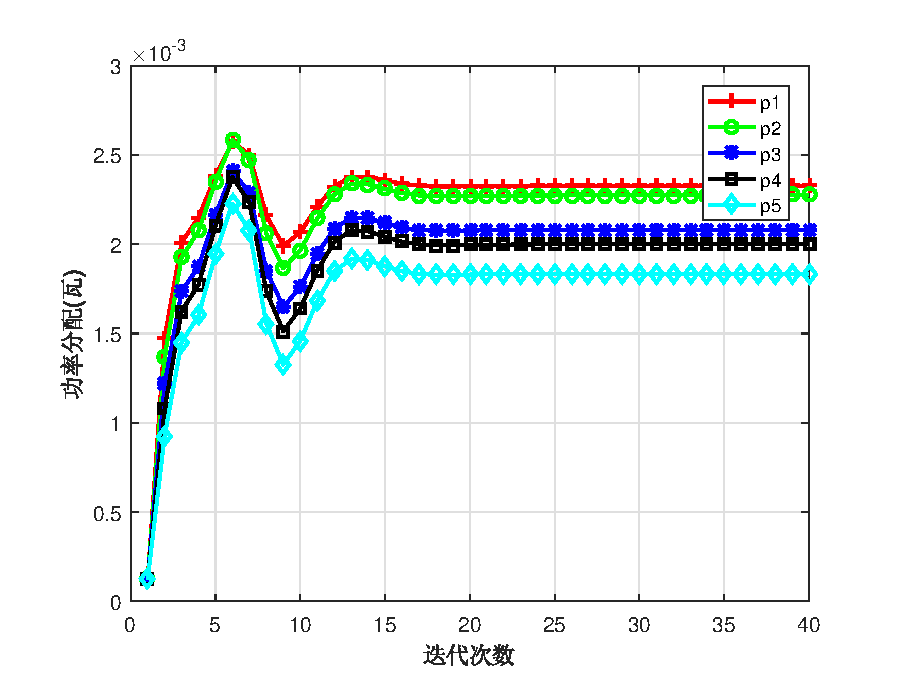
\includegraphics[width=10cm]{figures//chap3//pp.eps}
\caption{功率收敛性能}
\label{F2}
\end{figure}

图 \ref{F2} 和图 \ref{F3} 分别显示了算法3-1 中每个车载发射机的功率分配和云分配给RSU 的相应计算资源。从图中可以看出,云端分配的计算资源在第五次迭代时达到峰值,
并在达到云端总计算资源 $f_{total}$ 的限制后开始下降。由于鲁棒功率控制和任务卸载调度的计算资源分配,相应的计算资源分配也发生了变化。

图 \ref{F4} 显示了联合优化时系统总效用的收敛情况。从图中可以看出,网络系统总效用的收敛趋势与功率分配和计算率分配有关。观察到这一现象是合理的,因为方程 \eqref{E12} 给出了 $U$ 的定义。随着功率矢量 $\mathbf{p}$ 的增加,$R_i$ 也会对数增加,从而导致边际收益递减。因此,随着迭代次数的增加,效用值的增量会越来越小,最终导致效用值趋于稳定。当功率矢量$\mathbf{p}$ 和分子部分的执行效用$t_{i,exe}$ 随着计算功率矢量$\mathbf{f}$ 的增加而成反比减少时,$U$ 的分母会减少,分子会随着矢量$\mathbf{f}$ 的增加而增加。
\begin{figure}[H]
\centering
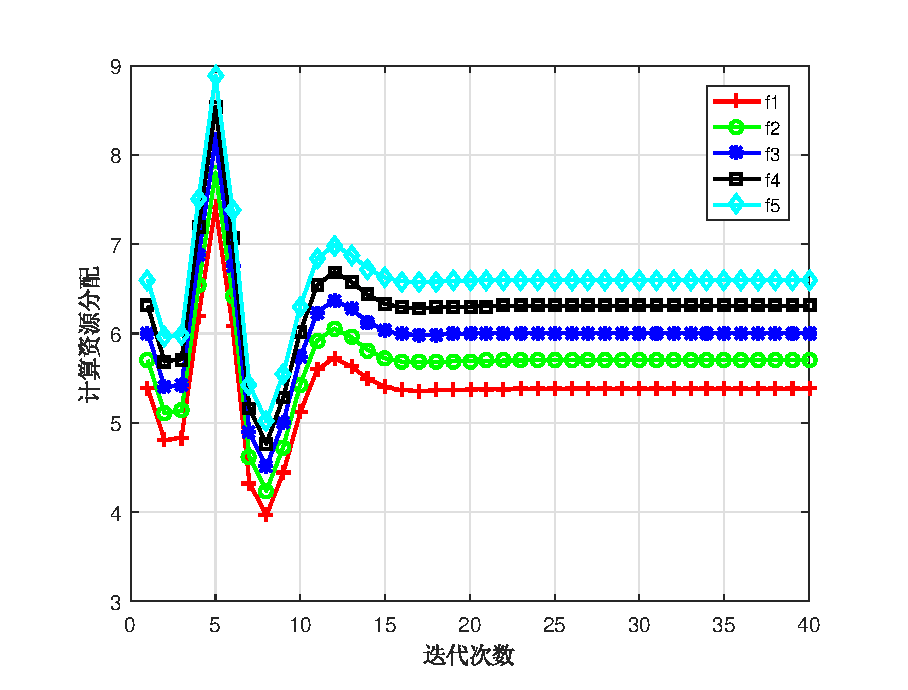
\includegraphics[width=10cm]{figures//chap3//ff.eps}
\caption{分配给RSU 的计算资源分配的收敛.}
\label{F3}
\end{figure}

\begin{figure}[H]
\centering
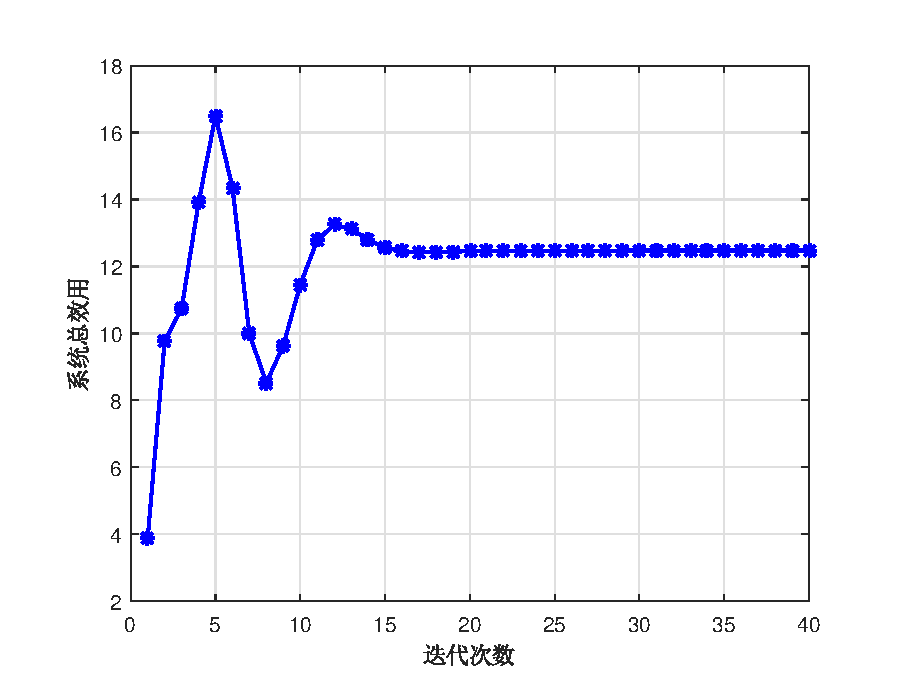
\includegraphics[width=10cm]{figures//chap3//ee.eps}
\caption{系统总效用的收敛.}
\label{F4}
\end{figure}

在支持 MEC 的车载云系统中,有必要考虑车辆的移动性。接下来,我们探讨了车辆移动对系统性能的影响。我们假设在指定时间段内车辆速度的任何变化都是微不足道的。为了进一步明确速度引起的多普勒频移对系统性能的影响,我们模拟了在系统中车辆速度恒定的条件下,基准值与增速测量值之间的比较。

图 \ref{F5} 展示了高流动性车辆环境下不同速度对系统性能的影响。
车辆环境下不同速度对系统性能的影响。由于 V2R 链路中的相对速度为零,且同一网络中所有车辆的速度相同,因此不存在多普勒效应。如图 \ref{F5} 所示,通信过程中的车速分别设置为20 m/s、30 m/s、40 m/s、50 m/s 和60 m/s。 因为车速越快,网络内的多普勒频移越大,这反过来又会导致信道不确定性增加,效用值随之下降。
\begin{figure}[H]
\centering
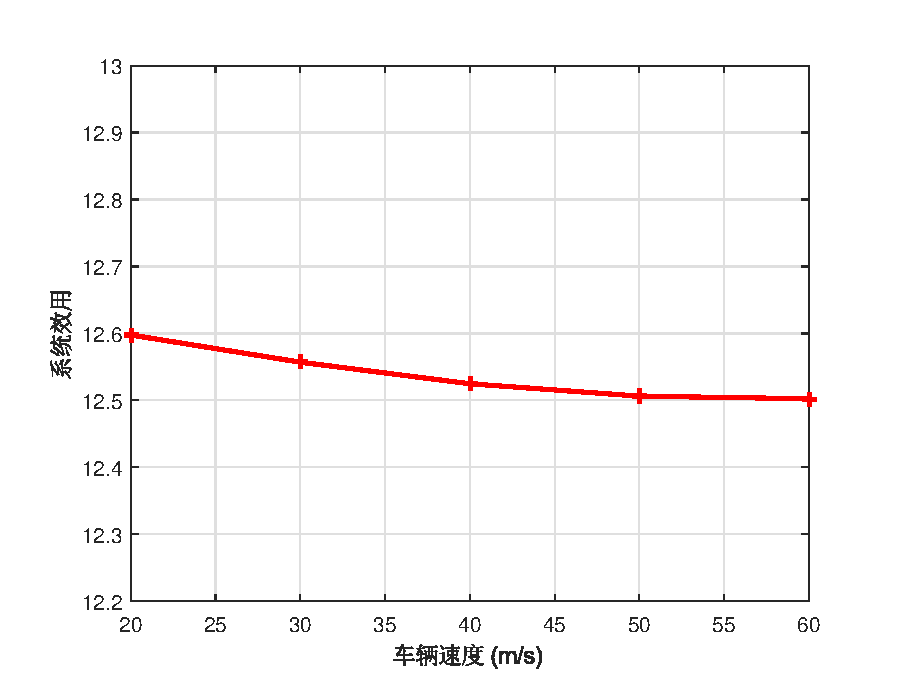
\includegraphics[width=10cm]{figures//chap3//diffspeed1.eps}
\caption{不同速度下系统总效用的对比.}
\label{F5}
\end{figure}

\begin{figure}[H]
\centering
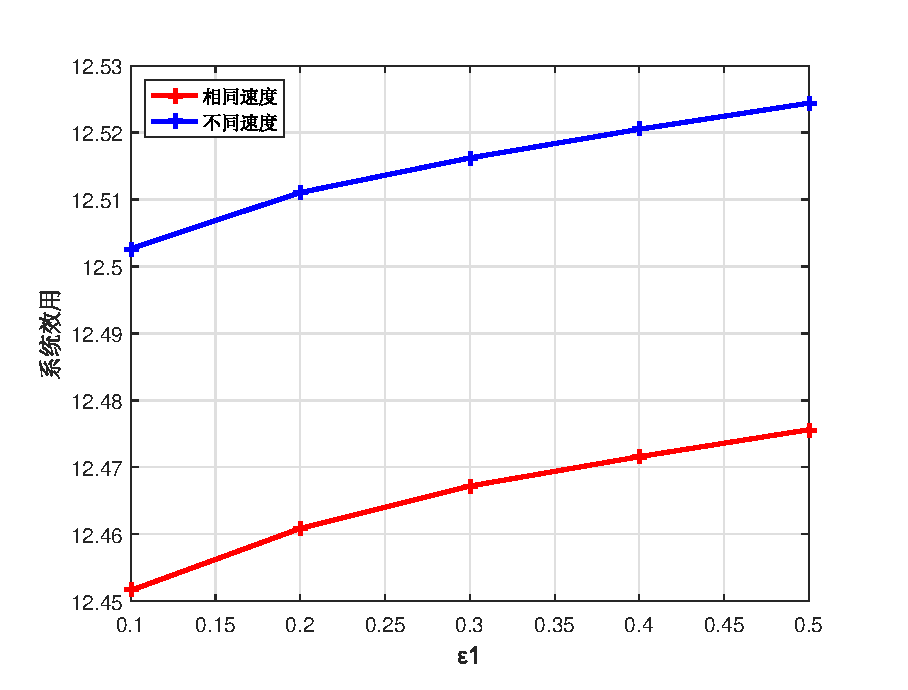
\includegraphics[width=10cm]{figures//chap3//diff_e1.eps}
\caption{不同 $\varepsilon_1$ 下系统总效用的变化.}
\label{F6}
\end{figure}

在考虑了车辆的流动性之后,进一步验证了所提方案的性能。图 \ref{F6} 显示了在使用不同的$\varepsilon_1$ 时,每辆车的相同速度和不同速度对总效用的影响。从图中可以看出,当 $\varepsilon_1$ 发生变化时,系统效用也会发生变化。每辆车在不同速度下的效用都高于所有车辆在相同速度下的效用。这一结果说明所提出的方法在复杂动态车辆网络中实施时具有很高的鲁棒性。

在计算率分配方面,我们选择默认的任务输入大小为 $d_u=420$KB (可参考 \cite{Xu2015})。它试图展示我们提出的算法的收敛性能。仿真结果表明,我们提出的方法优于三种基准方案。基准方案描述如下,
\begin{comment}
\begin{itemize}
\item[1)] 独立卸载和功率控制"(简称 "IOP"),即车辆独立执行功率控制和计算率分配,而不考虑彼此的最优值。
\item[2)] 在 " 无车辆功率控制"(简称 "Without-VPC")情况下,车辆的发射功率设定为卸载期间的平均功率。
\item[3)] 无计算速率分配"(表示为 "Without-CRA"),即在卸载过程中将云的计算速率分配设为固定值。
    %Similar to [?]Jiang2016  Similar to: \cite{Jiang2016},
\end{itemize}
\end{comment}

(1) 独立卸载和功率控制"(简称 "IOP"),即车辆独立执行功率控制和计算率分配,而不考虑彼此的最优值。

(2) 在 " 无车辆功率控制"(简称 "Without-VPC")情况下,车辆的发射功率设定为卸载期间的平均功率。

(3) 无计算速率分配"(表示为 "Without-CRA"),即在卸载过程中将云的计算速率分配设为固定值。

图 \ref{F7} 显示了不同情况下系统总效用的迭代收敛情况,图中显示鲁棒联合优化性能优于其他三种方案。从图中可以看出,四种方法在迭代后期都收敛到了一个稳定的值,其中建议方案的性能最好。

为了反映更真实的情况,每辆车所需的 CPU 任务负载(Megzcycles)往往不同,因此我们将五辆车的 CPU 任务负载(Megzcycles)分别设置为 1600、1700、1800、1900 和 2000。

\begin{figure}[H]
\centering
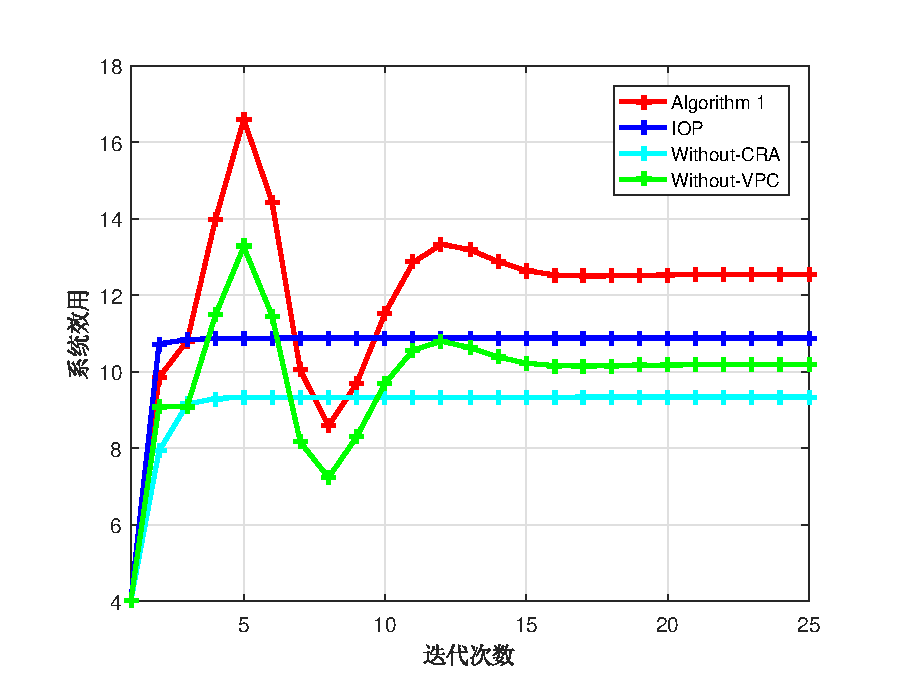
\includegraphics[width=10cm]{figures//chap3//compare.eps}
\caption{不同方案下系统总效用的收敛.}
\label{F7}
\end{figure}

从 \ref{F7} 可以看出,随着迭代次数的增加,车辆的平均系统效用逐渐发生变化并趋于稳定。在独立优化过程中,首先进行的是计算率分配,此时还不知道最优功率分配。采用功率和计算率交替优化的方法,每次迭代都能得到相应的最优值。单独优化首先优化功率向量 $\mathbf{p}$。 得到结果后,利用该结果优化计算率分配,然后优化计算率,得到系统。但是,如果采用联合优化,则两个变量都能达到最优值。
\begin{figure}[H]
\centering
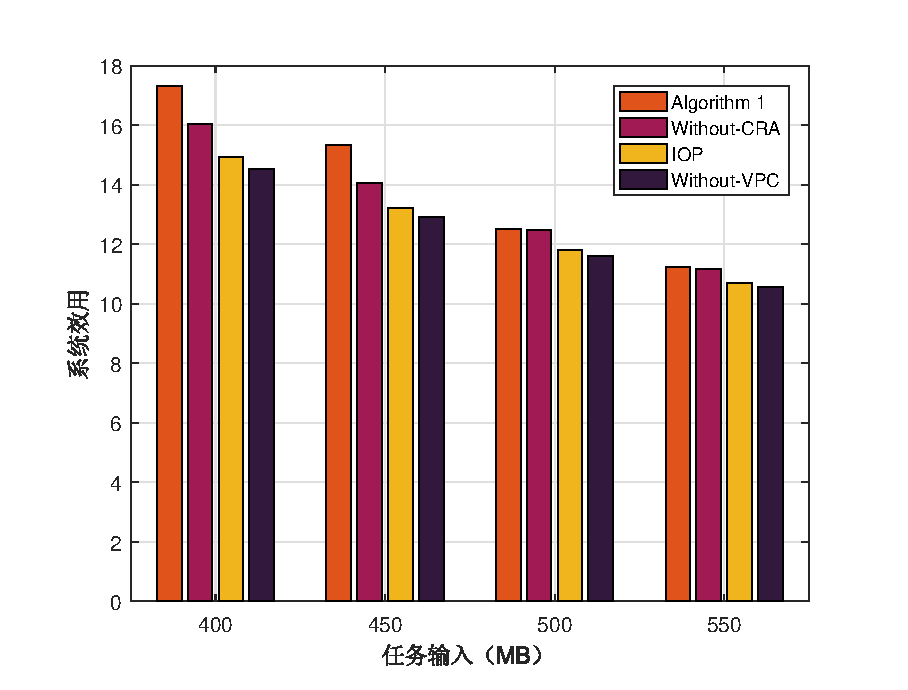
\includegraphics[width=10cm]{figures//chap3//diff_dup.eps}
\caption{不同输入数据 $d_u$ 下的系统效用.}
\label{F8}
\end{figure}
\begin{figure}[H]
\centering
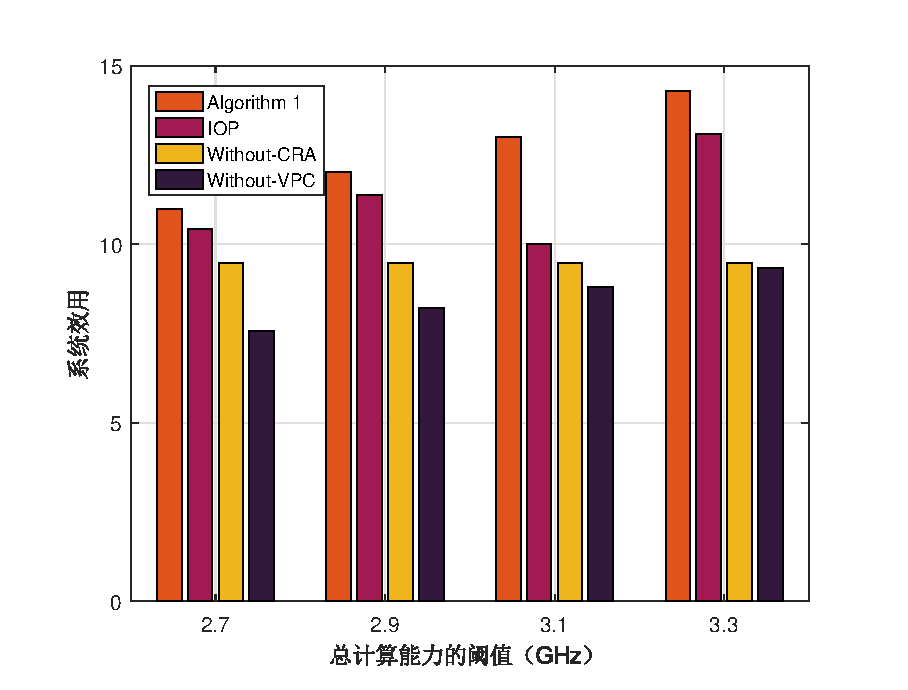
\includegraphics[width=10cm]{figures//chap3//diff_total.eps}
\caption{不同计算能力约束下的 $f_{total}$ 系统效用.}
\label{F9}
\end{figure}

图 \ref{F8} 中绘制了不同任务输入大小 $d_u$ 时四种竞争方案的平均系统效用。从图中可以看出,所有方案的平均系统效用都随着任务输入量的增加而降低。图中还显示,其他方案的性能增益也有类似的趋势。
这一现象是合理的,因为根据 \eqref{E12} 中 $U$ 的定义,工作量的增加会对系统性能产生负面影响。
图 \ref{F9} 显示了不同 $f_{total}$ 时的系统总成本比较。由于云的计算能力有限,当计算能力较小时,系统效用较小。
从图 \ref{F10} 中我们可以清楚地看到,当数据规模增大时,系统效用较小。当数据规模较大时,计算任务需要更多的上传时间。
\begin{figure}[H]
\centering
\includegraphics[width=10cm]{figures//chap3//diff_c.eps}
\caption{不同计算数据 $c_{i,e}$ 下的系统效用.}
\label{F10}
\end{figure}

\section{本章小结}\label{section3-5}
本章研究了车载网络中云辅助 MEC 的鲁棒功率控制和任务卸载的新方法。优化方案的目的是在最大化效用的同时保证车辆的 QoS。 由于信道存在不确定性,优化受到传输速率、计算通信延迟和同信道干扰概率形式的限制。最初的优化问题被表述为鲁棒性功率控制和任务卸载调度问题,很难解决。这里应用了 SCA 技术,将变量耦合的 NP 难问题转化为可处理的凸问题。鲁棒电源控制和任务卸载调度算法用于开发可行的解决方案。仿真结果表明,我们提出的算法得到了近似最优解。与现有方法相比,系统平均卸载效用得到显著改善。
\begin{comment}
\section{表格的引用}\label{section3-6}
表格的引用同样是使用\verb|\ref{}| 命令实现的。例如“表\verb|\ref{tab:ysubof}|” 输出的结果为:表\ref{tab:ysubof}。\LaTeX 会自动将其替换为表格的编号。例如:
\begin{verbatim}
燕山大学硕士学位论文参考文献规则的表格如表\ref{tab:ysubof} 所示。
\end{verbatim}
的效果如下:\\
燕山大学硕士学位论文参考文献规则的表格如表\ref{tab:ysubof} 所示。

\section{本章小结}\label{section3-7}
注意!从第二章开始应有`` 本章小结",主要总结本章所做的主要研究工作,研究成果等内容!!!

\end{comment}

%
